\section{Menu Phase: 2D Renderer}
With video system initialized, the game finally starts and displays the menu phase. It is look pretty simple but features a neat trick.
\par
\begin{figure}[H]
\centering
\includegraphics[width=\textwidth]{screenshots/first_menu.png}
\caption{Architecture and sub-systems.}
\end{figure}
\par

\begin{minipage}{.6\textwidth}
With control over the bank mask, it is actually possible to write multiple pixel (up to four) with one write operation. In the drawing to the right, pixels 0, 1, 2 and 3 are in different banks but at the same address (0x0000). By configuring the bank mak to all banks, it is possible to write these four pixels simulaneously.\\
To clear the screen to red before drawing the menu, the engine only takes 320x200/4 = 16,000 writes instead of 64,000.\\
\par
\end{minipage}
\begin{minipage}{.4\textwidth}
\begin{figure}[H]
\centering
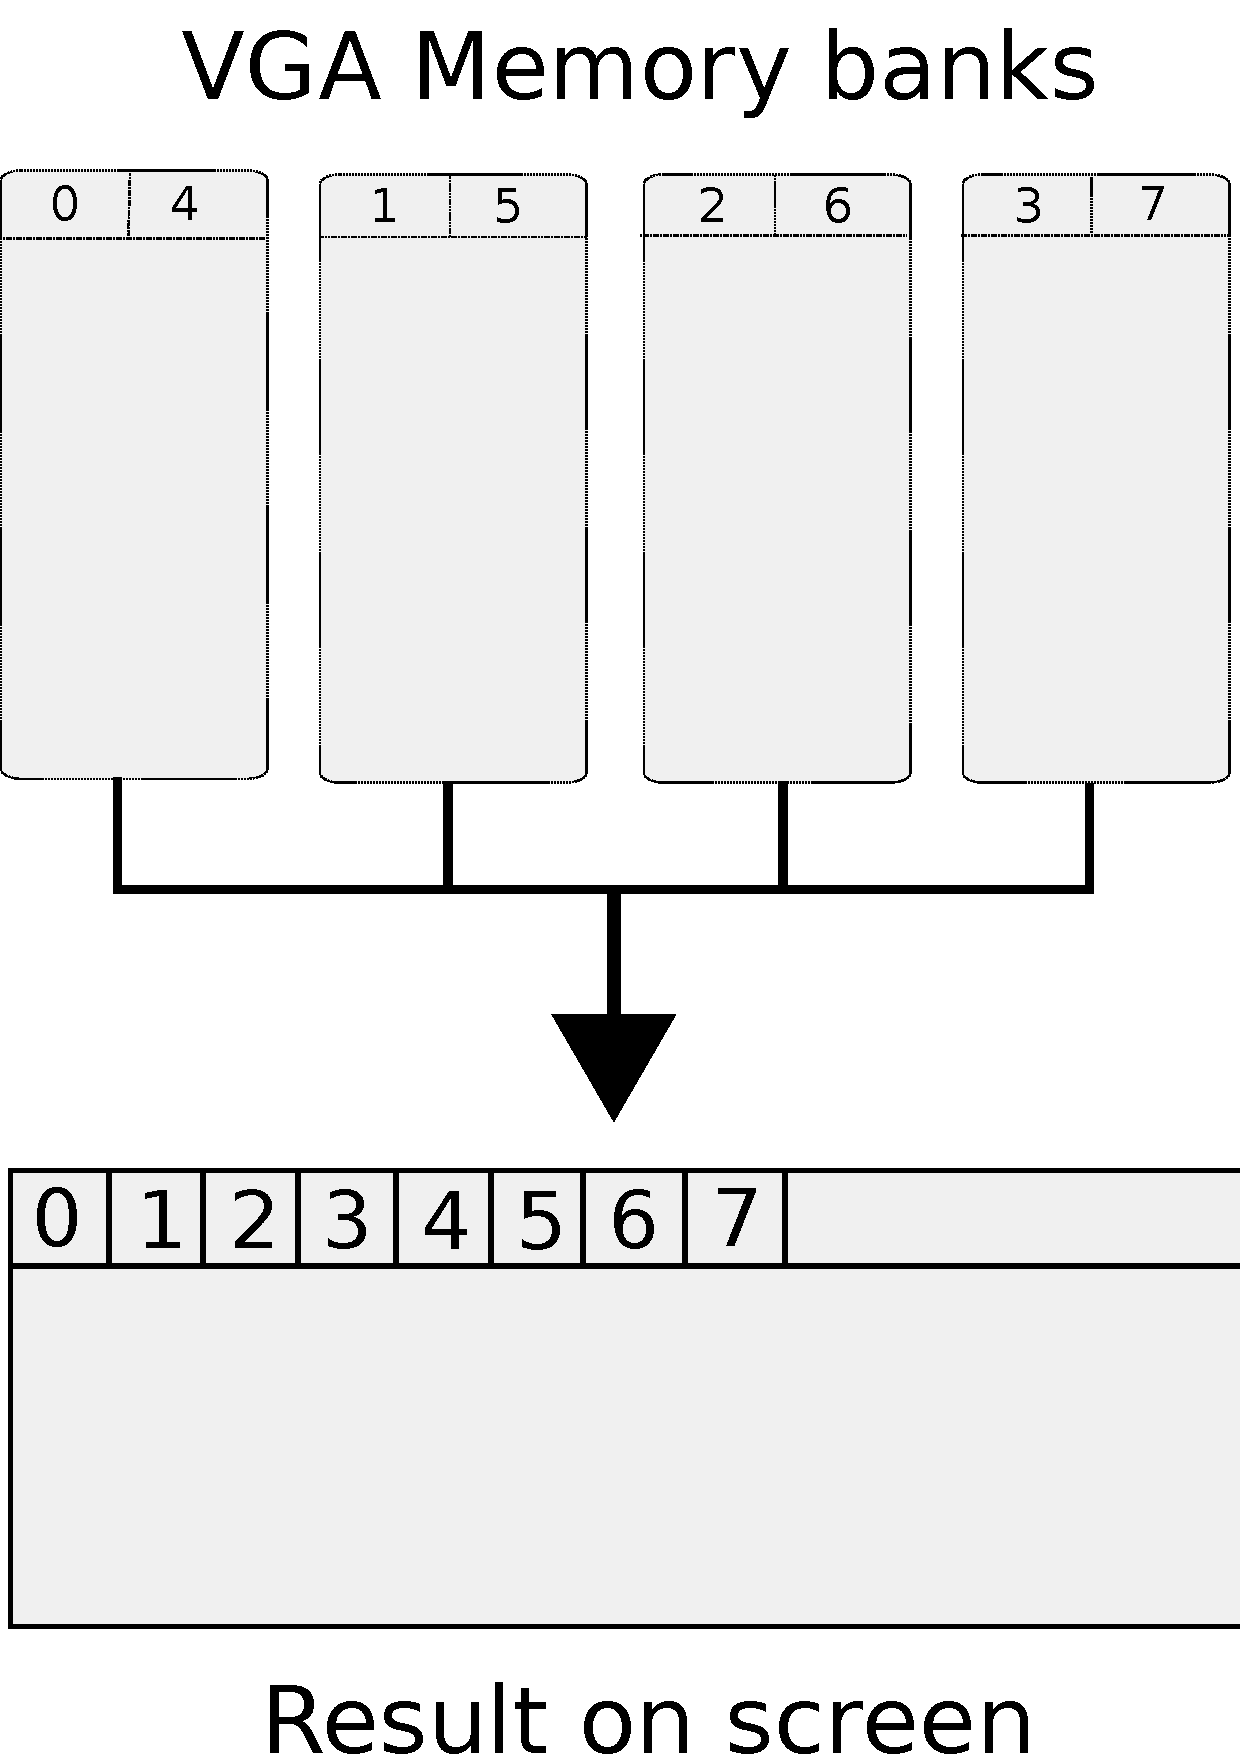
\includegraphics[width=\textwidth]{imgs/drawings/vga_ram_screen_layout.pdf}
\end{figure}
\end{minipage}



\lstinputlisting[language=C]{code/vga_clear/optimal.c}

There is a trick with this technique however: Only bytes at the same address in a bank can be populated.
\begin{figure}[H]
  \centering
 \includegraphics[width=\textwidth]{imgs/drawings/vga_multiple_pixel_write.png}
\end{figure}

The 2D renderer used extensively the US Manager to render font and the Cache manager to cache the assets.
Assets are called "pic" as opposed to sprites in 3D phases. Pics  are all Huffman-compressed (VGADICT, VGAHEAD, 
VGAGRAPH).
\par
\note{Where do i mention the bug with assets wrong id in meny (gun replaced by hero.)?}
Include code to write to all banks at the same time.

Not at fast as it seems since things have to be drawn in all three buffers during action 3D phase:\\
\par

\begin{minipage}{\textwidth}
\lstinputlisting[language=C]{code/StatusDrawPic.c}
\end{minipage}


LatchDrawPic
Chapter 48 from michael abrash book
atches were not intended for use in 256-color mode; that was something I figured out as a hack and wrote about. The latches were used so that in 16-color mode any or all of the four planes could be written to at once.

